\documentclass[11pt,letterpaper]{article}
\usepackage[T1]{fontenc}
\usepackage{lmodern,microtype}
\usepackage[margin=.85in,headheight=15pt]{geometry}
\usepackage{xcolor,booktabs,longtable,array,tabularx,enumitem,amsmath,graphicx,listings,tikz,fancyhdr,titlesec,hyperref,xurl}
\usetikzlibrary{arrows.meta,positioning,fit,shapes.geometric}
\definecolor{navy}{HTML}{16314D}\definecolor{teal}{HTML}{087F83}\definecolor{pale}{HTML}{EDF4F8}\definecolor{muted}{HTML}{536579}
\hypersetup{colorlinks=true,linkcolor=navy,urlcolor=teal,pdftitle={Comprehensive Architecture Analysis}}
\titleformat{\section}{\Large\bfseries\color{navy}}{\thesection}{.7em}{}
\titleformat{\subsection}{\large\bfseries\color{teal}}{\thesubsection}{.7em}{}
\pagestyle{fancy}\fancyhf{}\fancyhead[L]{\small Agent Harness Engineering}\fancyhead[R]{\small Technical study / v1.0}\fancyfoot[R]{\thepage}
\setlength{\parindent}{0pt}\setlength{\parskip}{5pt}\renewcommand{\arraystretch}{1.18}
\setlist{nosep,leftmargin=*}\newcolumntype{Y}{>{\raggedright\arraybackslash}X}
\newcommand{\src}[1]{\expandafter\nolinkurl\expandafter{\detokenize{#1}}}
\newcommand{\evidence}[1]{\par\smallskip{\small\raggedright\color{muted}\textbf{Source anchor:} #1\par}}
\tikzset{n/.style={draw=navy,rounded corners=2pt,fill=pale,align=center,minimum height=9mm,text width=31mm,font=\small},g/.style={n,draw=teal,fill=teal!7},edge/.style={-Latex,thick,draw=navy},boundary/.style={draw=teal,dashed,rounded corners,inner sep=5pt}}
\lstset{basicstyle=\small\ttfamily,breaklines=true,frame=single,backgroundcolor=\color{pale},columns=fullflexible,showstringspaces=false}
\begin{document}
\begin{titlepage}
\vspace*{1.25in}
{\color{teal}\large AGENT HARNESS COURSE STUDY / 01\par}\vspace{.3in}
{\color{navy}\Huge\bfseries Comprehensive Architecture Analysis\par}\vspace{.18in}
{\Large Components, control flows, memory and advanced execution patterns\par}\vspace{.5in}
\rule{\linewidth}{1pt}\par
\textbf{Source:} Richmond Alake's Harness Engineering for AI Agents course export\par
\textbf{Version:} 1.0 \quad 23 November 2026\par
\textbf{Status:} Technical study; not a production authorization\par
\vfill
The model proposes; the harness validates, governs, executes and records.
\end{titlepage}
\tableofcontents\clearpage
\section*{Reading note}
This standalone volume belongs to a six-document study of snapshot \src{8a5edab282632443}. Observed source behavior is distinguished from proposed controls. No live application, external provider or sandbox was independently executed. Test files are contract evidence, not independently verified passing results.

\section{Executive summary and scope}
The course is a memory-first, incremental implementation reference. Part 1 develops ERPA, a synthetic retail assistant, in packaged and custom forms. Part 2 introduces PPA, a personal productivity assistant whose actions can affect other people. Part 3 adds cost measurement, turn trajectories, skill learning and readiness checks. Advanced tracks cover durable workflows, research and metaharness evaluation. The architectural progression is an increase in operational responsibility, not merely model intelligence.

This study distinguishes \textbf{observed} source behavior from \textbf{proposed} production controls. The evidence is the supplied text snapshot (identifier \src{8a5edab282632443}), selected source code and tests, and the target curriculum README and roadmap fetched on 23 November 2026. Source paths refer to the supplied snapshot, not necessarily the latest upstream revision. The export contains text files and a tree; notebook bodies and external dependencies are not assumed available where absent. No upstream application, external provider or live sandbox was executed. Test files demonstrate intended contracts, not passing results. No exploit or production certification is claimed.

\begin{tabularx}{\linewidth}{p{.22\linewidth}YY}\toprule
Dimension & Strength & Production decision \\\midrule
Control loop & Explicit graph and interruption & Keep policy independent of graph and model \\
Memory & Multiple memory types, promotion, retrieval & Tenant-scoped provenance, retention and revocation \\
Tools & Allowlist, risk tiers, schemas & Least-privilege capability tokens at adapters \\
Durability & Checkpoints, restart demonstrations & Durable effect journal and reconciliation \\
Learning & Gate, version history and rollback & Isolated trials and independent release approvals \\
Evaluation & Frozen checks and fair comparison & Extend to adversarial, availability and isolation tests \\
\bottomrule\end{tabularx}
\section{Repository architecture analysis}
\subsection{Evolution across course parts}
\begin{center}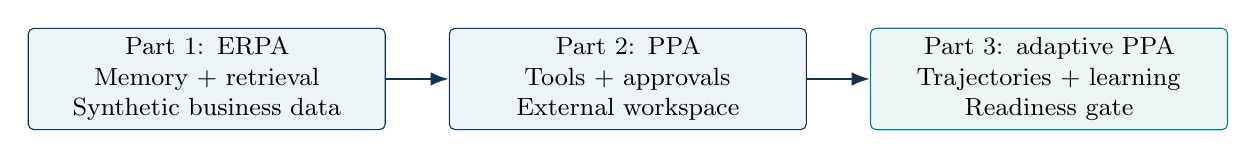
\begin{tikzpicture}[node distance=8mm]
\node[n,text width=43mm] (p1) {Part 1: ERPA\\Memory + retrieval\\Synthetic business data};
\node[n,text width=43mm,right=of p1] (p2) {Part 2: PPA\\Tools + approvals\\External workspace};
\node[g,text width=43mm,right=of p2] (p3) {Part 3: adaptive PPA\\Trajectories + learning\\Readiness gate};
\draw[edge] (p1)--(p2);\draw[edge] (p2)--(p3);
\end{tikzpicture}\end{center}
\textbf{Part 1.} Both implementations share fixtures, seed data and a recall--decide--write trace contract. The packaged MemoRizz path makes memory and tool abstractions accessible, while the custom path exposes graph construction, retrieval, semantic layer, scratch space, skills and tool execution. Local mode uses scripted deterministic behavior; optional live mode connects model providers, Oracle, MCP and sandbox services. The live custom graph in \src{langgraph_live.py} contains assemble context, call model, dispatch tools, finalize and persist; dispatch loops back through context assembly. The staged exercises move from single turn to memory, semantics, skills, tools and the complete harness. The pre-context semantic cache is an optimization, not an authority decision.
\evidence{\src{part_1/README.md}; \src{part_1/custom_harness/stages/}; \src{part_1/custom_harness/appbook/backend/core/langgraph_live.py}; \src{part_1/SPEC_COVERAGE.md}.}
\textbf{Part 2.} PPA adds real-world trust boundaries: incoming mail, calendar, contacts and notes; a practice workspace and optional real integrations; workspace gateway and MCP; governed definitions; focus timers, scheduled routines, event triggers; approval and safe mode. The second decision model (System One) screens attacks, ranks evidence and selects procedures/tools. Its output remains a signal rather than an authorization source. The pure policy functions define urgent, free slots, tracked tasks and recipient risk independently of the reasoning model.
\evidence{\src{part_2/_shared/runtime/policy.py}; \src{part_2/_shared/mcp/workspace_mcp_server.py}; \src{part_2/custom_harness/appbook/backend/core/}.}
\textbf{Part 3.} PPA retains the same operational structure and adds a token/cost ledger, per-turn trajectories, repeated workflow detection, candidate skill creation, a five-check promotion gate and a nine-check scorecard. The learning code selects live turns with qualifying outcomes, no existing skill, a recorded typed turn and nonempty tool signature. A repeated signature alone is not proof of safety. Skill activation is separate from candidate creation and gate results.
\evidence{\src{part_3/README.md}; \src{part_3/custom_harness/appbook/backend/core/learning.py}; \src{ledger.py}; \src{trajectories.py}; \src{scorecard.py} (same core directory).}
\subsection{Component responsibilities and dependencies}
\begin{longtable}{p{.22\linewidth}p{.35\linewidth}p{.35\linewidth}}\toprule
Component & Responsibility & Source examples \\\midrule\endhead
Ingress/API & Request, transcript, resume, inspection & Appbook backend routers; frontends \\
Agent engine & State graph, bounded model loop, tool dispatch & Part 1 \src{langgraph_live.py}; Part 3 \src{agent.py} \\
Model adapter & Provider calls and response normalization & \src{llm_client.py}; advanced \src{model_provider.py} \\
Context assembler & Stable prompt, memory, skills, available tools & \src{agent.py}, \src{skills.py}, \src{scratchfs.py} \\
Semantic layer & Governed domain facts and definitions & Part 1 \src{semantic.py}; Part 2 policy and \src{governed.py} \\
Tool registry & Discover, validate, invoke allowed operations & \src{tools.py}; workspace MCP server \\
Policy/approval & Effect tier, recipient risk, draft, decision, delivery & \src{approval.py}; shared \src{policy.py} \\
Persistence & Run/thread state, memory, action log and checkpoints & \src{store.py}, \src{oracle_store.py}; advanced \src{persistence.py} \\
Scheduler/runtime & Timers, routines, event triggers & \src{scheduler.py}, \src{runtime.py}, \src{events.py} \\
Evaluation & Trace and cost evidence, gate decisions & \src{ledger.py}, \src{scorecard.py}, \src{learning.py} \\
\bottomrule\end{longtable}
\subsection{Architectural patterns and tradeoffs}
\begin{longtable}{p{.24\linewidth}p{.32\linewidth}p{.36\linewidth}}\toprule
Pattern & Course example & Tradeoff \\\midrule\endhead
Single agent loop & ERPA and PPA model/tool cycles & Flexible; requires bounds and validation \\
Graph workflow & Advanced Part 1 risk review routes & Explicit control; schema migration and replay complexity \\
Router/dispatcher & System One selection and semantic registries & Smaller contexts; selection errors and hidden capabilities \\
Orchestrator--worker & Parallel research agents and writing fan-out & Coverage and throughput; correlated errors, cost and leakage \\
Evaluator--optimizer & Research reflection, review and revision & Quality gains only if evaluation and budgets are credible \\
Human-in-the-loop & PPA effects and research review gates & Prevents silent external changes; introduces wait state and fatigue \\
Metaharness & Part 1 MetaHarness and Part 2 packaged examples & Common evidence interface; wrapper differences can confound comparisons \\
Event-driven runtime & Timers and routines & Work survives request; needs ownership, leases and cancellation \\
\bottomrule\end{longtable}
\subsection{Turn lifecycle and data flows}
Part 3's \src{agent.py} assembles context, calls the model, dispatches validated tools, drafts effects, interrupts at human review, applies effects, calls the model again, and persists. Automatic tools and gated tools follow distinct paths. Approval decisions are written separately from delivery results. In contrast to Part 1's repeated context assembly, Part 3 aims to assemble stable context once and track provider prompt caching. The graph checkpoint is not itself a transaction with external mail or calendar services.
\begin{center}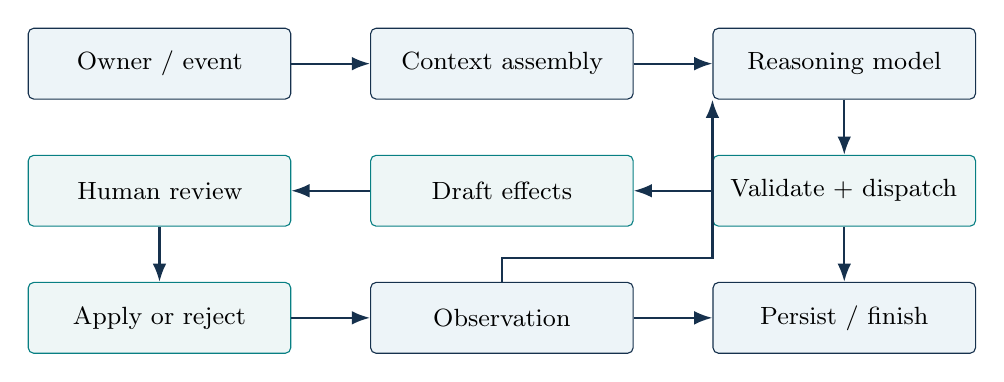
\begin{tikzpicture}[node distance=7mm and 10mm]
\node[n] (req) {Owner / event};\node[n,right=of req] (ctx) {Context assembly};\node[n,right=of ctx] (model) {Reasoning model};
\node[g,below=of model] (disp) {Validate + dispatch};\node[g,left=of disp] (draft) {Draft effects};\node[g,left=of draft] (review) {Human review};
\node[g,below=of review] (apply) {Apply or reject};\node[n,right=of apply] (obs) {Observation};\node[n,right=of obs] (persist) {Persist / finish};
\draw[edge](req)--(ctx);\draw[edge](ctx)--(model);\draw[edge](model)--(disp);\draw[edge](disp)--(draft);\draw[edge](draft)--(review);\draw[edge](review)--(apply);\draw[edge](apply)--(obs);\draw[edge](disp)--(persist);\draw[edge](obs)--(persist);\draw[edge](obs.north)--++(0,3mm)-|(model.south west);
\end{tikzpicture}\end{center}
\textit{Figure 1. Logical turn flow. The observation is supplied to the model for another bounded iteration; persistence may occur at checkpoints and on termination. The direct dispatch-to-persist edge summarizes the automatic/final path, not an exact graph edge.}
\subsection{Memory and context engineering}
\begin{tabularx}{\linewidth}{p{.23\linewidth}YY}\toprule
Memory & Content & Required lifecycle \\\midrule
Working & Current scratch, task plan, context window & Session-scoped, bounded, expires \\
Episodic & Past interactions and outcomes & Owner-scoped, redacted, time-stamped \\
Semantic & Facts, evidence, domain meaning & Provenance, freshness, conflict handling \\
Procedural & Skills and workflow recipes & Immutable versions, review and rollback \\
\bottomrule\end{tabularx}

The course uses scratch working memory and promotion to longer-term stores, with content-hash deduplication described in the PPA appbook. Distinguish raw evidence from extracted claims and approved instructions. Retrieval selects candidates, reranks and builds a bounded context; it never grants authority. Semantic cache hits are not prompt-cache hits: the former reuse a previous answer based on matching semantics, the latter reuse provider computation over a stable prefix. Never reuse authorization decisions, private data across principals, or an effectful completion on semantic similarity alone. The proposed cache key includes tenant, principal/scope, source versions, policy version, skill revision and model configuration; effectful requests bypass answer reuse.
\evidence{Part 1 \src{cache.py}, \src{retriever.py}, \src{semantic.py}; Part 3 \src{scratchfs.py}, \src{memory.py}, \src{ledger.py}.}
\subsection{Advanced modes}
The Part 1 advanced workflow documents a 17-node graph with missing-evidence, quick and parallel high-risk branches, Oracle checkpointing, semantic tool and skill registries and workflow promotion. The research track uses six MemAgents, private/shared Oracle memory, Tavily retrieval and governed E2B execution. The MetaHarness normalizes runs across model wrappers and records evidence; the separate fair evaluation notebook controls task samples and provider differences. Total Recall adds ontology/GraphRAG and governed semantic registries. These are documented implementations, not verified external services.

Part 3 research is a separate graph, not simply the assistant with a longer prompt. Its \src{graph.py} scopes a paper, interrupts for outline approval, gathers evidence, tallies, reflects, organizes, fans out writing, reviews, assembles and interrupts for publication review. Reflection is constrained by thin evidence, remaining rounds, new sources and budget. A blocked release permits an explicit override in source; production should restrict override authorization and record justification, or prohibit it for hard safety failures.
\begin{center}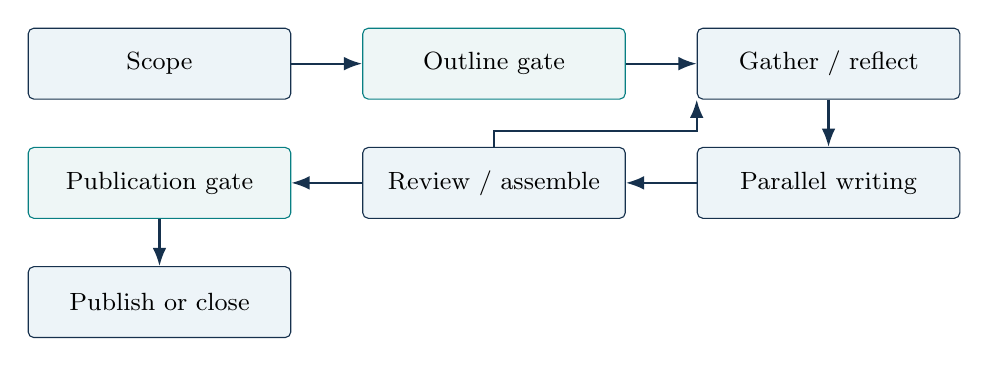
\begin{tikzpicture}[node distance=6mm and 9mm]
\node[n] (s) {Scope};\node[g,right=of s] (a) {Outline gate};\node[n,right=of a] (r) {Gather / reflect};\node[n,below=of r] (w) {Parallel writing};\node[n,left=of w] (v) {Review / assemble};\node[g,left=of v] (p) {Publication gate};\node[n,below=of p] (o) {Publish or close};
\draw[edge](s)--(a);\draw[edge](a)--(r);\draw[edge](r)--(w);\draw[edge](w)--(v);\draw[edge](v)--(p);\draw[edge](p)--(o);\draw[edge](v.north)--++(0,2mm)-|(r.south west);
\end{tikzpicture}\end{center}
\evidence{\src{part_1/advanced/README.md}; \src{part_1/advanced/INSTRUCTOR_RUNBOOK.md}; \src{part_3/advanced/deep_research/appbook/backend/harness/graph.py}, \src{budget.py}, \src{evidence.py}.}
\section{Source register and limitations}
\begin{itemize}
\item Richmond Alake, \textit{Harness Engineering for AI Agents}, supplied repository export,\newline snapshot \src{8a5edab282632443}; root README, Part 1--3 READMEs, code paths cited throughout. Workshop: \url{https://www.oreilly.com/live-events/harness-engineering-for-ai-agents/0642572381264}.
\item Target curriculum, README and roadmap, inspected 23 November 2026: \url{https://github.com/Notoriousjayy/agent-engineering-curriculum}.
\item Target documentation library, root README and AI technical-documents directory, inspected 23 November 2026: \url{https://github.com/Notoriousjayy/latex-docs}.
\end{itemize}
All figures are original logical reconstructions or proposed design diagrams; they are not copies of source graphics. Vendor-neutral controls, ADRs, acceptance tests and laboratory extensions are recommendations rather than claims about source implementation. Live dependencies, source test outcomes, provider claims, licensing/publication clearance and deployment configuration require separate validation.
\end{document}
